%%%%%%%%%%%%%%%%%%%%%%%%%%%%% Define Article %%%%%%%%%%%%%%%%%%%%%%%%%%%%%%%%%%
\documentclass{article}
%%%%%%%%%%%%%%%%%%%%%%%%%%%%%%%%%%%%%%%%%%%%%%%%%%%%%%%%%%%%%%%%%%%%%%%%%%%%%%%

%%%%%%%%%%%%%%%%%%%%%%%%%%%%% Using Packages %%%%%%%%%%%%%%%%%%%%%%%%%%%%%%%%%%
\usepackage[utf8]{inputenc}
\usepackage{array, float, geometry, amssymb, amsthm, amsmath, amsfonts}
\usepackage{graphicx, color, colortbl, wrapfig, parskip, caption, tabularx}
\usepackage[breaklinks]{hyperref}
\usepackage[table]{xcolor}
\usepackage{fancyhdr, psfrag, pgfplots, cite, lastpage}
\usepackage[english]{babel}
\usepackage{listings, mdframed, matlab-prettifier, hyperref}
\usepackage{lipsum, bookmark, booktabs, empheq, titlesec, verbatim, subfig, pdfpages, comment}

%%%%%%%%%%%%%%%%%%%%%%%%%%%%%%%%%%%%%%%%%%%%%%%%%%%%%%%%%%%%%%%%%%%%%%%%%%%%%%%

%%%%%%%%%%%%%%%%%%%%%%%%%% C Code Listing Settings %%%%%%%%%%%%%%%%%%%%%%%%%%%%%%%%%%%%%%%
\definecolor{mGreen}{rgb}{0.25,0.63,0.15}
\definecolor{mGray}{rgb}{0.5,0.5,0.5}
\definecolor{mPurple}{rgb}{0.58,0,0.82}
\definecolor{codeBlue}{rgb}{0.01, 0.2, 0.92}
\definecolor{codegray}{rgb}{0.5,0.5,0.5}
\definecolor{codepurple}{rgb}{0.58,0,0.82}
\definecolor{codeblue}{rgb}{0.13,0.29,0.53}
\definecolor{backgroundColour}{rgb}{0.95,0.95,0.95}
\definecolor{headercolor}{rgb}{0.212,0.502,0.955} 
\definecolor{rowcolor1}{rgb}{0.9, 0.9, 0.9}
\definecolor{rowcolor2}{rgb}{1, 1, 1}

\lstset{
    backgroundcolor=\color{backgroundColour},   
    commentstyle=\color{deepGreen},
    keywordstyle=\color{blue},
    numberstyle=\tiny\color{mGray},
    stringstyle=\color{red},
    basicstyle=\ttfamily\small,
    breakatwhitespace=false,
    breaklines=true,
    captionpos=b,
    keepspaces=true,
    numbers=left,
    numbersep=5pt,
    showspaces=false,
    showstringspaces=false,
    showtabs=false,
    tabsize=2,
    language=C,
    frame=single
}

%%%%%%%%%%%%%%%%%%%%%%%%%%%%%%%%%%%%%%%%%%%%%%%%%%%%%%%%%%%%%%%%%%%%%%%%%%%%%%%

% Other Settings
\hypersetup{
    colorlinks = true,
    linkcolor = black,
    urlcolor = blue,
}
\urlstyle{same}

%%%%%%%%%%%%%%%%%%%%%%%%%% Page Setting %%%%%%%%%%%%%%%%%%%%%%%%%%%%%%%%%%%%%%%
\geometry{a4paper}
\pagestyle{fancy}
\fancyhead{}
\fancyhead[L]{CS232 - Operating Systems}
\fancyhead[C]{Assignment 04 - Report}
\fancyhead[R]{}
\fancyfoot{}
\fancyfoot[C]{Page \thepage \;of 14}

%%%%%%%%%%%%%%%%%%%%%%%%%% Define some useful colors %%%%%%%%%%%%%%%%%%%%%%%%%%
\definecolor{ocre}{RGB}{243,102,25}
\definecolor{mygray}{RGB}{243,243,244}
\definecolor{deepGreen}{RGB}{26,111,0}
\definecolor{shallowGreen}{RGB}{235,255,255}
\definecolor{deepBlue}{RGB}{61,124,222}
\definecolor{shallowBlue}{RGB}{235,249,255}
%%%%%%%%%%%%%%%%%%%%%%%%%%%%%%%%%%%%%%%%%%%%%%%%%%%%%%%%%%%%%%%%%%%%%%%%%%%%%%%

%%%%%%%%%%%%%%%%%%%%%%%%%% Define an orangebox command %%%%%%%%%%%%%%%%%%%%%%%%
\newcommand\orangebox[1]{\fcolorbox{ocre}{mygray}{\hspace{1em}#1\hspace{1em}}}
%%%%%%%%%%%%%%%%%%%%%%%%%%%%%%%%%%%%%%%%%%%%%%%%%%%%%%%%%%%%%%%%%%%%%%%%%%%%%%%

%%%%%%%%%%%%%%%%%%%%%%%%%%%% English Environments %%%%%%%%%%%%%%%%%%%%%%%%%%%%%
\newtheoremstyle{mytheoremstyle}{3pt}{3pt}{\normalfont}{0cm}{\rmfamily\bfseries}{}{1em}{{\color{black}\thmname{#1}~\thmnumber{#2}}\thmnote{\,--\,#3}}
\newtheoremstyle{myproblemstyle}{3pt}{3pt}{\normalfont}{0cm}{\rmfamily\bfseries}{}{1em}{{\color{black}\thmname{#1}~\thmnumber{#2}}\thmnote{\,--\,#3}}
\theoremstyle{mytheoremstyle}
\newmdtheoremenv[linewidth=1pt,backgroundcolor=shallowGreen,linecolor=deepGreen,leftmargin=0pt,innerleftmargin=20pt,innerrightmargin=20pt,]{theorem}{Theorem}[section]
\theoremstyle{mytheoremstyle}
\newmdtheoremenv[linewidth=1pt,backgroundcolor=shallowBlue,linecolor=deepBlue,leftmargin=0pt,innerleftmargin=20pt,innerrightmargin=20pt,]{definition}{Definition}[section]
\theoremstyle{myproblemstyle}
\newmdtheoremenv[linecolor=black,leftmargin=0pt,innerleftmargin=10pt,innerrightmargin=10pt,]{problem}{Problem}[section]
%%%%%%%%%%%%%%%%%%%%%%%%%%%%%%%%%%%%%%%%%%%%%%%%%%%%%%%%%%%%%%%%%%%%%%%%%%%%%%%

\title{{\huge \textbf{Habib University \\ Operating Systems - CS232 }}

\vspace*{5mm}
{\LARGE \textbf{Assignment 04 - Report} \\ \textbf{Multi-Threading}}
{
\includegraphics[width=0.75\linewidth]{logo.png}} \\ 
{\Large \textbf{Instructor:} Munzir Zafar}}
\author{Ali Muhammad Asad - aa07190}
\date{}

\pgfplotsset{compat=1.18}

\begin{document}
\maketitle

\newpage
\tableofcontents

\newpage
\section{Introduction}
The assignment aims to use the knowledge of multi-threading using POSIX Threads API to use and implement a multi-threaded-file processor. The goal is to develop a multi-threaded C program that processes a large dataset concurrently. Therefore, synchronization mechanisms will be needed to ensure thread safety and efficient resource utlization

% \newpage	
\section{Makefile and I/O}
\subsection{Input}
\subsubsection*{Single Threaded Program}
The program takes one additional command line argument; the first one obviously being the name of the program, and the second command line argument will be the name of the data file to be processed. The data file name can also be a path to the directory in which the file is located, or the file can be in the same directory. If the user fails to provide the desired number of arguments, the program will exit with an error message. The program will also exit with an error message if the file provided is not found.

\subsubsection*{Multi-Threaded Program}
The program takes two additional command line arguments; the first one obviously being the name of the program, the second command line argument again being the name of the data file to be processed, and the third command line argument being the number of threads to launch for processing. If the user does not provide the number of threads, then the default value of 4 threads is used for processing. If the user fails to provide the desired number of arguments, the program will exit with an error message. The program will also exit with an error message if the file provided is not found.

\subsection{Makefile}
The accompanying makefile has also been provided with the program and supports the following commands: \vspace*{-2mm}
\begin{mdframed}
  \begin{itemize}
    \item[-] \texttt{make build:} builds the program and generates the executable files titled \texttt{``fps''} (file processor single thread) and \texttt{``fpm''} (file processor multi-thread) \vspace*{-1mm}
    \item[-] \texttt{make runs <input\_file>:} runs the single threaded program with the given dataset file.  \vspace*{-1mm}
    \item[-] \texttt{make runm <input\_file> [num\_threads]:} runs the multi-threaded program, with the given dataset file, and provided number of threads. \vspace*{-1mm}
    \item[-] \texttt{make clean:}  cleans the directory by removing the executable files \vspace*{-1mm}
  \end{itemize}
\end{mdframed}
\newpage
\section{Implementation}
\subsection{Data Structres}
\subsubsection*{Single Threaded Program}
In the single threaded program, the primary data structure being used is a dynamically allocated array \texttt{``data''} that stores the integer data of the file.
\begin{lstlisting}[caption={Dynamic Data Array}]
typedef long long int ll;
ll *data; ll cap = 10;
data = (ll *)malloc(cap * sizeof(ll));
/* Code ... */
  cap *= 2;
  data = (ll*)realloc(data, cap * sizeof(ll));
  /* More Code */
\end{lstlisting}
As we are parsing over a huge data set (maybe even more than the sample), the data array is of type ``\texttt{long long int}'' to prevent integer overflows. Additionally, a \texttt{cap} was used that is updated if the dataset reaches the capacity of the array, in which case, the cap increases and the array is reallocated to double of its size. This is a common strategy that balances the time spent between frequent allocations and memory overhead.
% This simple python program shows the final cap of the array and the number of times we needed to dynamically re-allocate the array, which is quite nice and efficient in terms of overhead.
% \begin{figure}[htbp]
%   \centering
%   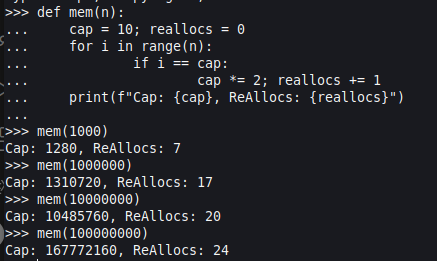
\includegraphics[width = 0.75\textwidth]{allocs.png}
%   \caption{Dynamic Array Allocation}
% \end{figure}
% \pagebreak
\subsubsection*{Multi-Threaded Program}
\begin{enumerate}
  \item \textbf{Data Array:} The data array in the multi-threaded prgram remains the same as it was in the single threaded program, with the same logic for dynamic re-allocation.
  \item \textbf{Thread Data Struct:} A thread data struct was created that would point to the data set, and marks the starting and ending points of the data set that the thread would be processing. Therefore, it encapsulates the data each thread performs its computation on.
        \begin{lstlisting}[caption={Thread Data Struct}]
typedef struct{
  ll* data;
  ll start;
  ll end;
} threadData;\end{lstlisting}

  \item \textbf{Thread Arrays:} Two distinct arrays were used; one that would store the thread identifiers of each worker thread, and one that would keep track of the thread data struct to pass individual thread-specific data.
        \begin{lstlisting}[caption={Thread Arrays}]
pthread_t threads[num_threads];
threadData thread_data[num_threads];
\end{lstlisting}
        The \texttt{thread\_data} is initialized with the data array, and the starting and ending points of the data set that each thread would be processing. The \texttt{threads} array is initialized with the thread identifiers of each thread. They work in tandem to ensure that each thread has the data it needs to process, and the thread identifier to be able to join the thread later on.

  \item \textbf{Mutex:} Lastly, two ``\texttt{mutex}'' of type \texttt{pthread\_mutex\_t}; \texttt{mutex\_sum} and \texttt{mutex\_minmax} were used to provide a mechanism for synchronizing access to shared global variables. This would ensure that updates to the global variables are thread-safe, preventing rac conditions.
\end{enumerate}
% \newpage
\subsection{Algorithms and Code}
\subsubsection{Single Threaded Program}
\begin{lstlisting}[caption={Single Threaded Program} label={lst:single}]
#include<stdio.h>
#include<stdlib.h>
#include<time.h>
#include<limits.h>

#define ITERS 100
typedef long long int ll; 

int main(int argc, char *argv[]){
  if (argc != 2){ // Check if the number of arguments is correct
    printf("Usage: %s <input_file>\n", argv[0]); return 1;
  }
  clock_t start = clock(); // Start timer for reading file
  FILE *datafile = fopen(argv[1], "r"); // Open file in read mode
  if(datafile == NULL){ // Check if file exists
    fprintf(stderr, "Error: Could not open file %s. Please check if the file with the given name exists\n", argv[1]); return 1;
  }

  // Allocate memory for data
  ll *data, *temp; ll size = 0, cap = 1000;
  data = (ll *)malloc(cap * sizeof(ll));
  if(data == NULL){ // Check if memory allocation was successful
    fprintf(stderr, "Error: Memory allocation failed!\n");
    fclose(datafile); return 1;
  }

  // While there is data in the file, add it to the integer array
  while(fscanf(datafile, "%lld", &data[size]) == 1){
    size++; // Increment size
    if(size == cap){ // If size is equal to capacity, double the capacity and dynamically reallocate memory
      cap *= 10;
      temp = (ll *)realloc(data, cap * sizeof(ll));
      if(temp == NULL){ // Check if memory reallocation was successful
        fprintf(stderr, "Error: Memory allocation failed!\n");
        free(data); fclose(datafile); return 1;
      } data = temp; // If successful, assign the new memory location to data
    }
  } fclose(datafile); 
  // End timer for reading file and print the time taken
  clock_t end = clock();
  double elapsed_time = (double)(end - start) / CLOCKS_PER_SEC;
  printf("Time taken to read file: %lf\n", elapsed_time);

  // Calculating sum, min and max values of the data set
  double sum_time = 0, minmax_time = 0; ll sum, min, max;
  // Run the function ITERS times and calculate the average time taken for sum, and, minimum and maximum
  for(size_t j = 0; j < ITERS; j++){
    clock_t start_sum = clock(); sum = 0;
    for(int i = 0; i < size; i++) sum += data[i];
    clock_t end_sum = clock();
    sum_time += (double)(end_sum - start_sum) / CLOCKS_PER_SEC;
  }
  for(int j = 0; j < ITERS; j++){
    clock_t start_minmax = clock();
    min = LLONG_MAX; max = LLONG_MIN;
    for(int i = 0; i < size; i++){
      if(data[i] > max) max = data[i];
      if(data[i] < min) min = data[i];
    }
    clock_t end_minmax = clock();
    minmax_time += (double)(end_minmax - start_minmax) / CLOCKS_PER_SEC;
  }

  printf("Sum: %lld \t Min: %lld \t Max: %lld\n", sum, min, max);
  printf("Average time taken to calculate sum: %lf\n", sum_time / ITERS);
  printf("Average time taken to calculate min and max: %lf\n", minmax_time / ITERS);
  
  // Free the memory allocated to data
  free(data); 
  return 0;
}
\end{lstlisting}
The listing above shows the single threaded program code. It starts by checking if the suer has provided the correct number of arguments, and its correctness. It then proceeds to open the file provided by the user, reading it line by line, and storing the data in the dynamically allocated array. Once the file has been read, the program proceeds to parse over the data set, first computing the sum of the data, and calculating the average time taken to compute the sum. It then proceeds to compute the minimum and maximum of the data set, and calculates the average time taken to compute the minimum and maximum. The average time taken is calculated by running the same computation 100 times, and taking the average of the time taken across these 100 runs. The program then frees the dynamically allocated array, and exits.
% The above listing shows the single threaded program code. The program starts by checking if the user has provided the correct number of command line arguments. If not, the program exits with an error message. If the user has provided the correct number of command line arguments, the program proceeds to open the file provided by the user. If the file is not found, the program exits with an error message. If the file is found, the program proceeds to read the file line by line, and stores the data in the dynamically allocated array. The array is dynamically allocated as necessary. Once the file has been read, the program proceeds to parse over the data set, as per the \texttt{parseData()} function, and computes the sum, minimum, and maximum of the data set. The program then proceeds to compute the average time taken to compute the sum, minimum, and maximum of the data set [\textit{for the average, the same computation was done 10 times, and the average was taken across these times}]. The program then frees the dynamically allocated array, and exits.
\pagebreak
\subsubsection{Multi-Threaded Program}
\begin{lstlisting}[caption={Multi-Threaded Program} label={lst:multi}]
#include<stdio.h>
#include<stdlib.h>
#include<time.h>
#include<pthread.h>
#include<limits.h>

#define ITERS 100
#define DEFAULT_NUM_THREADS 4

typedef long long int ll;

// Global Shared Variables
ll global_sum = 0, global_min = LLONG_MAX, global_max = LLONG_MIN;

// Mutex for synchronization
pthread_mutex_t mutex_sum, mutex_minmax;

// Thread Data Structure
typedef struct{
  ll* data;           // Pointer to the data array
  ll start;           // Start index of the chunk
  ll end;             // End index of the chunk
} threadData;

void* compSum(void* arg){
  threadData* tdata = (threadData*) arg;
  ll* data = tdata->data; // Pointer to the data array
  ll sum = 0;
  for(size_t i = tdata->start; i < tdata->end; i++) sum += data[i];
  // Update global variables
  pthread_mutex_lock(&mutex_sum);
  global_sum += sum;
  pthread_mutex_unlock(&mutex_sum);
  pthread_exit(NULL);
}

void* compMinMax(void* arg){
  threadData* tdata = (threadData*) arg;
  ll* data = tdata->data; // Pointer to the data array
  ll min = LLONG_MAX, max = LLONG_MIN;
  for(size_t i = tdata->start; i < tdata->end; i++){
    if(data[i] > max) max = data[i];
    if(data[i] < min) min = data[i];
  }
  // Update global variables
  pthread_mutex_lock(&mutex_minmax);
  if(min < global_min) global_min = min;
  if(max > global_max) global_max = max;
  pthread_mutex_unlock(&mutex_minmax);
  pthread_exit(NULL);
}

int main(int argc, char* argv[]){
  // Check if the number of arguments is correct
  if(argc < 2 || argc > 3){
    fprintf(stderr, "Usage: %s <input_file> [num_threads] where num_threads is optional, if not provided, the default is 4\n", argv[0]); return 1;
  }
  int num_threads = DEFAULT_NUM_THREADS; // Default number of threads
  if(argc == 3){ // If number of threads is provided, check if it is valid
    num_threads = atoi(argv[2]);
    if(num_threads < 1){
      fprintf(stderr, "Error: Invalid number of threads\n"); return 1;
    }
  }
  clock_t file_start = clock(); // Start timer for reading file
  FILE* datafile = fopen(argv[1], "r");
  if(datafile == NULL){ // Check if file exists
    fprintf(stderr, "Error: Could not open file %s. Please check if the file with the given name exists\n", argv[1]);
    return 1;
  }

  // Allocate memory for data
  ll* data, *temp; ll size = 0, cap = 100;
  data = (ll*)malloc(cap * sizeof(ll));
  if(data == NULL){ // Check if memory allocation was successful
    fprintf(stderr, "Error: Memory allocation failed!\n");
    fclose(datafile); return 1;
  }
  
  // While there is data in the file, add it to the integer array
  while(fscanf(datafile, "%lld", &data[size]) == 1){
    size++; // Increment size
    if(size == cap){ // If size is equal to capacity, double the capacity and dynamically reallocate memory
      cap *= 10;
      temp = (ll*)realloc(data, cap * sizeof(ll));
      if(temp == NULL){ // Check if memory reallocation was successful
        fprintf(stderr, "Error: Memory allocation failed!\n");
        free(data); fclose(datafile); return 1;
      } data = temp; // If successful, assign the new memory location to data
    }
  } fclose(datafile);
  // End timer for reading file and print the time taken
  clock_t file_end = clock();
  double file_read = (double)(file_end - file_start) / CLOCKS_PER_SEC;
  printf("Time taken to read file: %lf\n", file_read);

  // Initialize mutexes
  pthread_mutex_init(&mutex_sum, NULL); pthread_mutex_init(&mutex_minmax, NULL);
  double sum_time = 0, minmax_time = 0; // Time taken to calculate sum, min and max
  // Run the function ITERS times and calculate the average time taken for sum, and, minimum and maximum
  pthread_t threads[num_threads]; // Array of threads
  threadData thread_data[num_threads]; // Array of thread data
  ll chunk_size = size / num_threads; // Size of each chunk
  for(int i = 0; i < num_threads; i++){
    thread_data[i].data = data;
    thread_data[i].start = i * chunk_size;
    thread_data[i].end = (i == num_threads - 1) ? size : (i + 1) * chunk_size;
  }
  struct timespec sum_start, sum_end, minmax_start, minmax_end;
  clock_gettime(CLOCK_MONOTONIC, &sum_start);
  for(int j = 0; j < ITERS; j++){
    global_sum = 0; 
    // Create and launch threads
    for(int i = 0; i < num_threads; i++) pthread_create(&threads[i], NULL, compSum, &thread_data[i]);

    // Wait for all threads to finish
    for(int i = 0; i < num_threads; i++) pthread_join(threads[i], NULL);
  }
  clock_gettime(CLOCK_MONOTONIC, &sum_end);
  sum_time = (double)(sum_end.tv_sec - sum_start.tv_sec) + (double)(sum_end.tv_nsec - sum_start.tv_nsec) / 1e9;

  clock_gettime(CLOCK_MONOTONIC, &minmax_start);
  for(int j = 0; j < ITERS; j++){
    global_min = LLONG_MAX; global_max = LLONG_MIN;
    // Create and launch threads
    for(int i = 0; i < num_threads; i++) pthread_create(&threads[i], NULL, compMinMax, &thread_data[i]);
    
    // Wait for all threads to finish
    for(int i = 0; i < num_threads; i++) pthread_join(threads[i], NULL);
  }
  clock_gettime(CLOCK_MONOTONIC, &minmax_end);
  minmax_time = (double)(minmax_end.tv_sec - minmax_start.tv_sec) + (double)(minmax_end.tv_nsec - minmax_start.tv_nsec) / 1e9;

  // Print the sum, min and max values, and the average time taken by each thread and the average elapsed time
  printf("Sum: %lld \t Min: %lld \t Max: %lld\n", global_sum, global_min, global_max);
  printf("Average time taken to calculate sum: %lf\n", sum_time / ITERS);
  printf("Average time taken to calculate min and max: %lf\n", minmax_time / ITERS);

  // Destroy the mutex and free the memory allocated to data
  pthread_mutex_destroy(&mutex_sum); pthread_mutex_destroy(&mutex_minmax);
  free(data);
  return 0;
}
\end{lstlisting}
The above listing shows the multi-threaded program code. After making the necessary checks, and populating the data into the array, the program initalizes two mutexes; one for the sum and one for min/max operation. It then proceeds to initialize the thread data struct and thread identifier arrays according to the number of threads; default or user provided. It then creates a chunk size of the data set that each thread would be processing. Then for each thread, we point its corresponding struct to the data array, and mark its starting and ending point in the array. Then we create each thread, and pass each thread data struct as an argument to the thread function responsible for computing the sum. Then those threads are joined once they've effectively calcualted their local sums, and updated the global sum variable. The start and end time for this computation is noted over 10 iterations of the same computation to get the average time taken to calcualte the sum. The same process is repeated to compute the minimum and maximum; a different function is used for computing minimum and maximum, and the average time across 100 iterations is noted. The program then frees the dynamically allocated array, and exits.
% The above listing shows the multi-threaded program code. After making the necessary checks and populating the data into the array, the program initializes the mutex, and proceeeds to initialize the thread data struct and thread identifier arrays according to the either the number of threads provided by the user, or the default value of 4. It then creates a chunk size of the data set that each thread would be processing. Then for each thread, we point its corresponding struct to the data array, and mark its starting and ending point in the array. Then we create the thread, and pass the thread data struct as an argument to the thread function. Once all threads have been created, we join them, and compute the average time taken to compute the sum, minimum, and maximum of the data set [\textit{for the average, the same computation was done 10 times, and the average was taken across these times}]. The program then frees the dynamically allocated array, and exits. The program returns two times, one that shows the average time taken by each thread, and the other that shows the average elapsed time. The average time taken by each thread is the time taken by each thread to compute the sum, minimum, and maximum of its chunk of the data set. The average elapsed time is the time taken by the program to compute the sum, minimum, and maximum of the entire data set.

\newpage
\section{Timing Comparison and Analysis}
\begin{mdframed}[backgroundcolor=shallowBlue]
  \textit{\textcolor{red}{*} The following timings were taken on a 4-core 8-Threads Intel i7-6700HQ CPU @ 3.50GHz, therefore, the performance may vary on different systems.}
\end{mdframed}

The timings were taken for 4 sample files; \texttt{data\_tiny} (1000 integers), \texttt{data\_small} (1000000 integers), \texttt{data\_medium} (10000000 integers), and \texttt{data\_large} (100000000 integers). For each of these data files, the single threaded program was run, and the multi-threaded program was run passing various number of threads as command line arguments. The average time for each program was taken across 10 runs.

\subsection{Single Threaded Program}
The table below summarizes the average elapsed time for each of the data sets on the single threaded program.
\begin{table}[h!]
  \centering
  \renewcommand{\arraystretch}{1.5} % Increase the row height
  \setlength\tabcolsep{8pt} % Increase the spacing between columns here
  \rowcolors{2}{rowcolor2}{rowcolor1} % Start alternating colors from the second row
  \begin{tabular}{|l|c|c|}
    \hline
    \rowcolor{headercolor}
    \textcolor{white}{\textbf{Dataset}} & \textcolor{white}{\textbf{Average Time - SUM}} & \textcolor{white}{\textbf{Average Time - MIN/MAX}} \\ \hline
    \textbf{data\_tiny} & 0.000015 & 0.000015 \\
    \textbf{data\_small} & 0.002580 & 0.002895 \\
    \textbf{data\_medium} & 0.025862 & 0.026871 \\
    \textbf{data\_large} & 0.258235 & 0.272356 \\ \hline
  \end{tabular}
  \caption{Timings for Single-Threaded Program}
  \label{tab:single_threaded_timings}
\end{table}

\vspace*{-5mm}
\subsection{Multi-Threaded Program}
The table below summarize the average time taken by a thread, and the average elapsed time of the multi-threaded program, on various number of threads for each data set.

\begin{figure}[htbp]
  \centering
  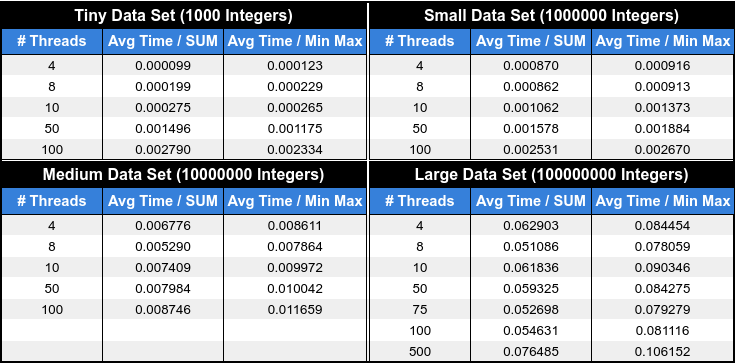
\includegraphics[width=1.0\textwidth]{multi.png}
  \label{fig:multitimes}
\end{figure} \vspace*{-5mm}
\begin{center}
  Table 2: Timings for Multi-Threaded Program on various number of threads
\end{center}

\subsection{Analysis}
The average time for sum is, in general, less than that for min/max. The sum operation is a sequential operation with no branching, thus can be easily pipelined. Finding the min/max involves comparison, which introduces branching, potentially causing pipeline stalls in the CPU. Addition is also generally faster than comparison. Also, accessing data sequentially can be cache friendly; for minimum and maximum, there is an additional overhead of comparison, thus increasing the time taken to compute the minimum and maximum.

\subsubsection*{Single vs Multi-Threaded}
For the tiny data set, the single threaded program performs better than the multi-threaded program. A reason could be that the overhead of thread creation, context switching, and synchronization outweighs the benefits of concurrent execution, as evident in the time elapsed for processing, which does not improve as the number of threads increase.

As the data set size increases, the single-threaded performance degrades, which is expected because the amount of computation increases with the size of the data. The multi-threaded, in general, shows a significant improvement in processing times. This suggests that the computational workload is enough to benefit from parallelization from multiple threads. The performance improvement also suggests good scalability, reflecting efficient parallelization; the multiple threads each get a portion of the data set available to operate on. Owing to concurrency, the time taken to compute the sum, and the minimum and maximum of the entire data set reduces significantly.

\subsubsection*{Multi-Threaded Performance in terms of Number of Threads}
\begin{figure}[htbp]
  \centering
  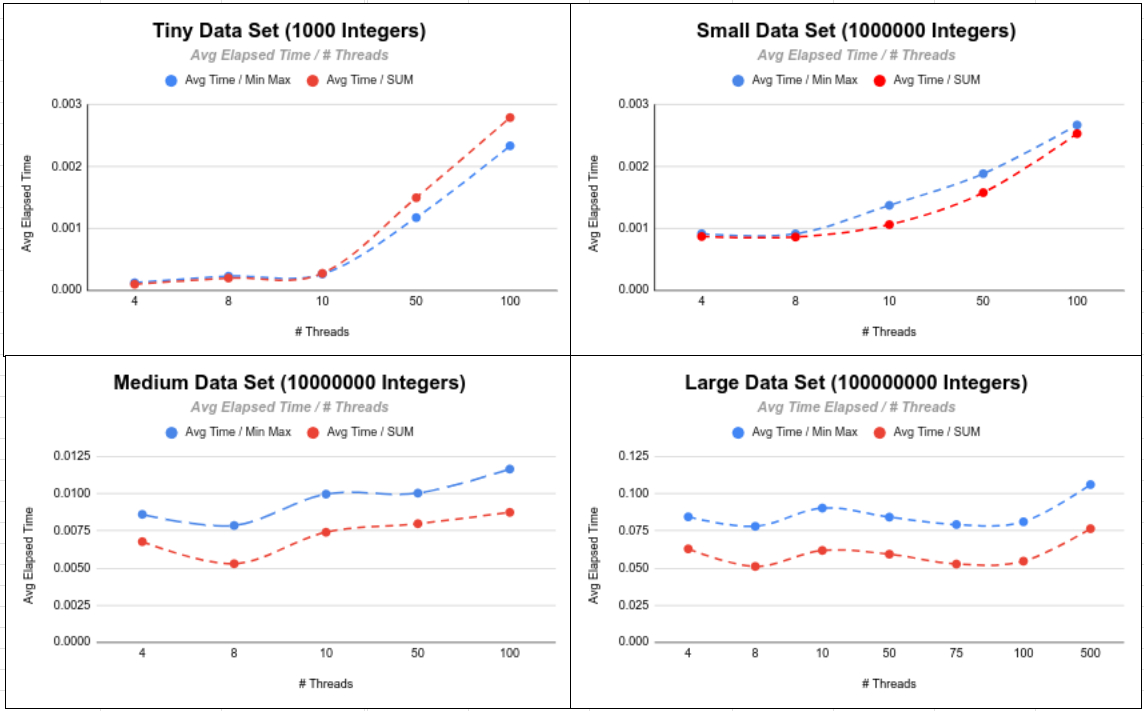
\includegraphics[width=1.0\textwidth]{multi_thread.png}
  \caption{Elapsed Time per \# of threads for varying data sets}
\end{figure}
The figure above summarizes the results of the \hyperref[fig:multitimes]{\textcolor{red}{multi-threaded table}} above.
For the tiny data set, the average elapsed time remains somewhat same up to 10 threads, after which there is a marked increase. This suggests that the overhead associated with thread management — such as creation, context switching, and synchronization — supercedes the execution time for computation of a such a tiny data set.  For the small data set, the same can be said, as we see a similar increasing trend in the average elapsed time after 8 threads. As the data set size increases, the benefits of multi-threading become more pronounced (apart from the fact that they outperform single threaded program by a significant amount) as we see a smaller increase (albiet an increase) in between average elapsed times as number of threads increases. This also suggests that there is an optimal thread count that aligns with the system'c core capabilities after which the performance degrades.

\textit{*My system has 4 cores with hyperthreading due to which we get 8 threads - 2 threads per core.}

The medium and large data sets exhibit the best performance on 8 threads as compared to 4 threads, likely due to the large computational workload which can effectively utilize the available logical threads provided by the 4 physical cores with hyper-threading (thus 8 threads) on this system. Beyond 8 threads we again see an increase in the average elapsed time, indicating that the performance is again diminshing with increasing threads mainly due to the system's capabilities as the cost of additional threads outweighs the computational benefit as more threads have to be managed by the cpu. This also underlines the importance of balancing thread count with actual core availability - and increasing threads doesn't necessarily imply an increase in overall performance.

In the large data set, however, we see a performance boost after 50 threads, and roughly upto 100 threads after which the performance starts to degrade again. While this does seem counter intuitive, this could be happening due to a variety of reasons for this specific number and on this specific data set. There might be a better cache utlization for certain operations, thus offsetting the overhead of context switching. The underlying thread library and OS scheduler may also have some optimizations that are triggered at this specific number of threads, that the large data set is benefitting from but not the others. The specific way the workload is distributed amongst threads can be a reason for better performance. It could also be due to hyperthreading; for such a large data set, if the threads are waiting on memory, which is common for large data sets, the CPU can switch to the other thread, improving overall throughput. Nonetheless, this is an interesting observation, and I would like to investigate this further.

Overall, the data, as shown in the figure above, indicates that 8 threads deliver the best performance on my system which is capable of running 8 threads simultaneously (seems logical).

\newpage
\section{Takeaway and Reflection}
This was the easiest assignment as of yet (thankfully), and a fun one. It was interesting to note that a balance must be kept in all things, even in thread count with actual core availability. Multi-threading does indeed lead to a better performance, but only to a certain extent. So there is an optimal thread count, closely tied to the system's hardware configuration.

\begin{figure}[htbp]
  \centering
  
\includegraphics[width=1.0\textwidth]{balance_best.jpeg}
\end{figure}

% \newpage
\section{References}
 [1] \textit{OpenAI.} ChatGPT [Online]. Available: \url{https://chat.openai.com/} mainly for commenting, and error resolving


\end{document}